\documentclass[tikz,border=5pt]{standalone}
\usepackage[UTF8,fontset=fandol]{ctex}
\usepackage{amsmath,amssymb}
\usetikzlibrary{arrows.meta,calc,patterns}
\tikzset{every picture/.style={>=Latex,line cap=round,line join=round,font=\small},
 dimension/.style={<->,thin,black!75},force/.style={->,very thick,red!75!black},
 guide/.style={dashed,thin,gray!70}}
\begin{document}

% 1: Preserve the oblique direction of the supplied problem drawing.
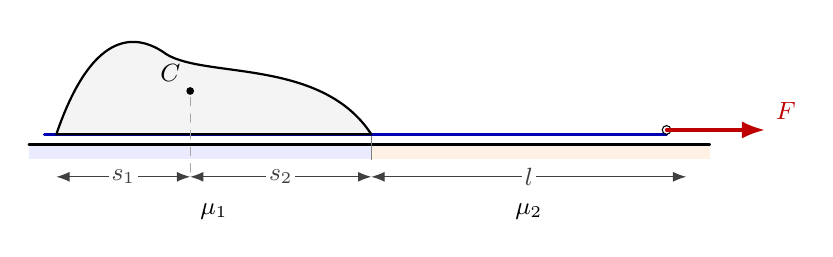
\begin{tikzpicture}
 \fill[blue!8] (-4.35,-.13) rectangle (0,-.32);
 \fill[orange!10] (0,-.13) rectangle (4.3,-.32);
 \draw[thick] (-4.35,-.13)--(4.3,-.13);
 \draw[gray] (0,-.32)--(0,-.02);
 \draw[blue!70!black,very thick] (-4.15,0)--(3.75,0);
 \filldraw[fill=gray!9,thick]
 (-4,0).. controls(-3.6,1.17)and(-3.1,1.34)..(-2.65,1.05)
 ..controls(-2.2,.69)and(-.65,1.0)..(0,0)--cycle;
 \fill (-2.3,.55) circle(1.4pt);
 \node[above left] at(-2.3,.55){$C$};
 \draw[guide](-2.3,.47)--(-2.3,-.53);
 \draw[dimension](-4,-.54)--(-2.3,-.54) node[midway,fill=white,inner sep=1pt]{$s_1$};
 \draw[dimension](-2.3,-.54)--(0,-.54) node[midway,fill=white,inner sep=1pt]{$s_2$};
 \draw[dimension](0,-.54)--(4,-.54) node[midway,fill=white,inner sep=1pt]{$l$};
 \node at(-2,-.98){$\mu_1$};
 \node at(2,-.98){$\mu_2$};
 \draw[fill=white] (3.75,.055) circle(.055);
 \draw[force](3.75,.055)--(5,.055) node[above right]{$F$};
\end{tikzpicture}

% 2: Conditional horizontal model. X=y-x; x is measured leftwards from right end.
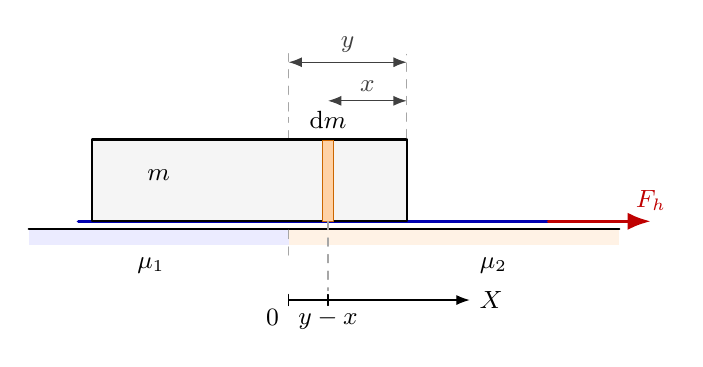
\begin{tikzpicture}
 \fill[blue!8](-3.3,-.10)rectangle(0,-.30);
 \fill[orange!10](0,-.10)rectangle(4.2,-.30);
 \draw[thick](-3.3,-.10)--(4.2,-.10);
 \draw[guide](0,-.43)--(0,1.32);
 \draw[blue!70!black,very thick](-2.67,0)--(3.3,0);
 \filldraw[fill=gray!8,thick](-2.5,0)rectangle(1.5,1.04);
 \filldraw[fill=orange!35,draw=orange!80!black](.43,0)rectangle(.57,1.03);
 \node at(-1.65,.58){$m$};
 \node[above] at(.5,1.06){$\mathrm dm$};
 \draw[dimension](.5,1.53)--(1.5,1.53) node[midway,above]{$x$};
 \draw[guide](1.5,1.06)--(1.5,2.12);
 \draw[dimension](0,2.02)--(1.5,2.02) node[midway,above]{$y$};
 \draw[guide](0,1.4)--(0,2.13);
 \draw[force](3.3,0)--(4.6,0) node[above]{$F_h$};
 \node at(-1.75,-.56){$\mu_1$};
 \node at(2.6,-.56){$\mu_2$};
 \draw[->](0,-1.0)--(2.3,-1.0) node[right]{$X$};
 \draw(0,-1.07)--(0,-.93);
 \node[below left]at(0,-1.0){$0$};
 \draw(.5,-1.07)--(.5,-.93);
 \node[below]at(.5,-1.0){$y-x$};
 \draw[guide](.5,0)--(.5,-.88);
\end{tikzpicture}

% 3: Domain 0<=x<=y<=l. Every drawn bound is used in the Fubini equations.
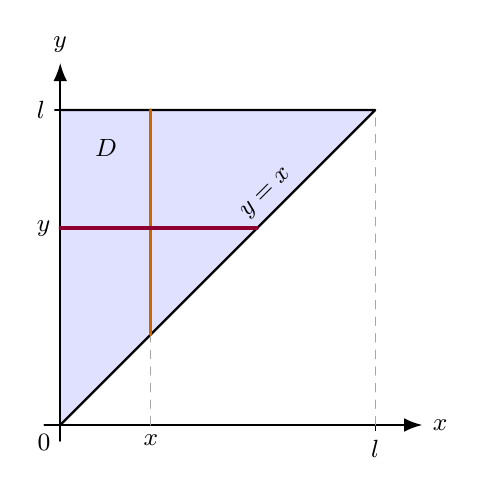
\begin{tikzpicture}
 \fill[blue!12](0,0)--(0,4)--(4,4)--cycle;
 \draw[->,thick](-.2,0)--(4.6,0)node[right]{$x$};
 \draw[->,thick](0,-.2)--(0,4.6)node[above]{$y$};
 \draw[thick](0,4)--(4,4)--(0,0);
 \node[below left]at(0,0){$0$};
 \draw(4,.07)--(4,-.07)node[below]{$l$};
 \draw(.07,4)--(-.07,4)node[left]{$l$};
 \draw[guide](4,0)--(4,4);
 \node[rotate=45,above]at(2.78,2.78){$y=x$};
 \draw[guide](1.15,0)--(1.15,1.15);
 \draw[orange!80!black,very thick](1.15,1.15)--(1.15,4);
 \node[below]at(1.15,0){$x$};
 \draw[purple!75!black,very thick](0,2.5)--(2.5,2.5);
 \node[left]at(0,2.5){$y$};
 \node at(.58,3.52){$D$};
\end{tikzpicture}

% 4: A single load element: left distance x and right distance l-x.
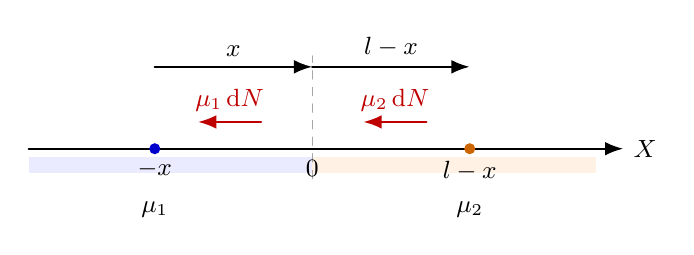
\begin{tikzpicture}
 \fill[blue!8](-3.6,-.10)rectangle(0,-.31);
 \fill[orange!10](0,-.10)rectangle(3.6,-.31);
 \draw[->,thick](-3.6,0)--(3.95,0)node[right]{$X$};
 \draw[guide](0,-.38)--(0,1.18);
 \fill[blue!80!black](-2,0)circle(2pt);
 \fill[orange!80!black](2,0)circle(2pt);
 \node[below]at(-2,-.03){$-x$};
 \node[below]at(0,-.03){$0$};
 \node[below]at(2,-.03){$l-x$};
 \draw[->,thick](-2,1.04)--(0,1.04)node[midway,above]{$x$};
 \draw[->,thick](0,1.04)--(2,1.04)node[midway,above]{$l-x$};
 \draw[->,red!75!black,thick](-.65,.34)--(-1.45,.34)node[midway,above]{$\mu_1\,\mathrm dN$};
 \draw[->,red!75!black,thick](1.45,.34)--(.65,.34)node[midway,above]{$\mu_2\,\mathrm dN$};
 \node at(-2,-.77){$\mu_1$};
 \node at(2,-.77){$\mu_2$};
\end{tikzpicture}

% 5: Only vertical forces shown; horizontal actions act on the same bottom line.
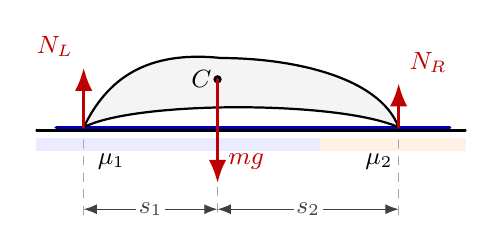
\begin{tikzpicture}
 \fill[blue!8](-3.6,-.10)rectangle(0,-.26);
 \fill[orange!10](0,-.10)rectangle(1.85,-.26);
 \draw[thick](-3.6,0)--(1.85,0);
 \draw[blue!70!black,very thick](-3.35,.04)--(1.65,.04);
 \filldraw[fill=gray!9,thick]
 (-3,.04)..controls(-2.7,.66)and(-2.2,1.02)..(-1.25,.92)
 ..controls(-.4,.92)and(.75,.7)..(1,.04)
 ..controls(.25,.38)and(-2.35,.38)..(-3,.04)--cycle;
 \fill(-1.3,.65)circle(1.5pt);
 \node[left,inner sep=2pt]at(-1.3,.65){$C$};
 \draw[force](-3,.04)--(-3,.799)node[above left]{$N_L$};
 \draw[force](1,.04)--(1,.601)node[above right]{$N_R$};
 \draw[force](-1.3,.65)--(-1.3,-.67)node[pos=.79,right]{$mg$};
 \draw[guide](-3,-.12)--(-3,-1.09);
 \draw[guide](1,-.12)--(1,-1.09);
 \draw[guide](-1.3,-.72)--(-1.3,-1.09);
 \draw[dimension](-3,-1.0)--(-1.3,-1.0)node[midway,fill=white,inner sep=1pt]{$s_1$};
 \draw[dimension](-1.3,-1.0)--(1,-1.0)node[midway,fill=white,inner sep=1pt]{$s_2$};
 \node at(-2.65,-.40){$\mu_1$};
 \node at(.75,-.40){$\mu_2$};
\end{tikzpicture}

% 6: Graph coordinate x is the material label, not the laboratory direction.
% Illustrative pressure: a=.45, b=.2, so centroid x/l=.575.
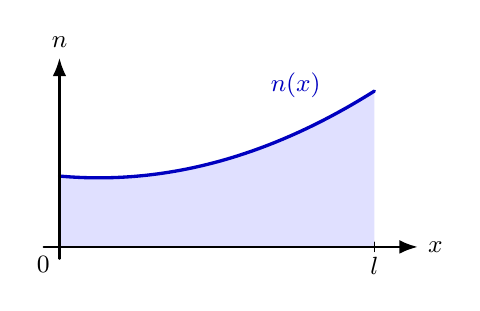
\begin{tikzpicture}
 \fill[blue!12]
 (0,0)--plot[domain=0:4,samples=101]
 (\x,{1.2*(1+.45*(2*\x/4-1)+.2*(6*(\x/4)^2-6*\x/4+1))})
 --(4,0)--cycle;
 \draw[blue!75!black,very thick]
 plot[domain=0:4,samples=101]
 (\x,{1.2*(1+.45*(2*\x/4-1)+.2*(6*(\x/4)^2-6*\x/4+1))});
 \draw[->,thick](-.2,0)--(4.55,0)node[right]{$x$};
 \draw[->,thick](0,-.15)--(0,2.4)node[above]{$n$};
 \draw(4,-.06)--(4,.06);
 \node[below]at(4,0){$l$};
 \node[below left]at(0,0){$0$};
 \node[blue!75!black]at(3.0,2.05){$n(x)$};
\end{tikzpicture}
\end{document}
